\documentclass[11pt,letterpaper,final]{report}
\usepackage[utf8]{inputenc}
\usepackage[english]{babel}
\usepackage{amsmath}
\usepackage{indentfirst}
\usepackage{amsfonts}
\addto{\captionsenglish}{\renewcommand{\bibname}{\LARGE{References}}}
\usepackage{pdfpages}
\usepackage{subcaption}
\usepackage{etoolbox}
\usepackage{amssymb}
\usepackage[font=small,labelfont=bf]{caption}
\usepackage{hanging}
\usepackage{notoccite}
\usepackage{float}
\usepackage{makeidx}
\usepackage{color}
\usepackage{graphicx}

\usepackage{multirow}


\usepackage{booktabs}% http://ctan.org/pkg/booktabs
\newcommand{\tabitem}{~~\llap{\textbullet}~~}


\usepackage{lscape}

\usepackage{enumitem}

\usepackage{titlesec}



\usepackage{gensymb}
\usepackage{hyperref}
\usepackage{graphicx}
\usepackage{lmodern}

\makeatletter
% section from book
%\newcommand\section{\@startsection {section}{1}{\z@}%
%                                   {-3.5ex \@plus -1ex \@minus -.2ex}%
%                                   {2.3ex \@plus.2ex}%
%                                   {\normalfont\Large\bfseries}}

\renewcommand\chapter{\@startsection {chapter}{0}{\z@}%
                                   {-1.5ex \@plus -1ex \@minus -.2ex}%
                                   {.5ex \@plus.2ex}% 
                                   {\normalfont\Large\textbf}}

 
\makeatletter

\renewcommand\section{\@startsection {section}{0}{\z@}%
                                   {-.1ex \@plus -1ex \@minus -.2ex}%
                                   {.05ex \@plus.2ex}% 
                                   {\normalfont\large\textbf}}


\makeatletter


\setlength{\parskip}{\baselineskip}%
\setlength{\parindent}{0pt}%






\usepackage{fourier}

\usepackage[left=1in,right=1in,top=1in,bottom=1in]{geometry}

\titleformat{\chapter}{\normalfont\huge}{\thechapter.}{20pt}{\huge\bf}
\titlespacing*{\chapter}{0pt}{-.5in}{20pt}
\author{Charles Hammond \\ Jaime Luo \\ Jacob Newman}


\begin{document}



\begin{center}

\begin{huge} 

\begin{Huge}\textbf{Work Plan} \end{Huge} \\~\\  Design of New UV System for UC Davis Wastewater Treatment Plant \\~\\
\end{huge}






\begin{large}

\vspace{100pt}

\includegraphics[height=1.5in]{wp1}\\
\end{large}
\begin{Large} \textit{pHlux Engineering} \\ \textit{Team 20} \end{Large}
\vspace{100pt}


\begin{tabular}{ll}
    \textbf{Prepared by:}&Charles Hammond\\
                         & Jaime Luo\\
                         & Jacob Newman\\
                         & \\~\\
    \textbf{Prepared for:}& UC Davis Utilities Division \\
                         & \\~\\
    \textbf{Finalized on:}& \today\\ 

\end{tabular}

\end{center}

\pagenumbering{gobble}


\newpage
\setcounter{page}{0}


%%%%%%%%%%%%%%%%%%%%%%%%%%%%%%%%%%%%%%%%%%%%%%%%%%%%%%%%%%%%%
%%%%%%%%%%%%%%%%%%%%% Executive Summary %%%%%%%%%%%%%%%%%%%%%
%%%%%%%%%%%%%%%%%%%%%%%%%%%%%%%%%%%%%%%%%%%%%%%%%%%%%%%%%%%%%


\chapter*{Executive Summary}
\pagenumbering{roman} 

    \addcontentsline{toc}{chapter}{Executive Summary}

    On January 11th, 2019, the UC Davis Utilities Division (Utilities Division) contacted pHlux Engineering to request assistance in solving two problems affecting the UC Davis Wastewater Treatment Plant (WWTP). The plant treats its effluent with ultraviolet (UV) disinfection, but often violates the minimum UV transmissivity (UVT) of 55\% required by the plant’s National Pollutant Discharge Elimination System (NPDES) permit. The Utilities Division has requested that pHlux Engineering investigate the recurring UVT violations and potentially recommend that the Central Valley Regional Water Quality Board (CVRWQCB) modify the requirement in the plant’s NPDES permit. Additionally, the current UV disinfection system is approaching the end of its useful life and a replacement design has been requested. 

This work plan defines the problems to be addressed, the project objectives, the technical approach, and the project management strategies that will be used to achieve those objectives. The deliverables for this project include a technical memorandum addressed to the CVRWQCB with recommendations for modifying the UVT requirement in the NPDES permit by April 5, 2019; a presentation of the final disinfection system design on May 19, 2019; a final poster to be presented at the Senior Design Showcase on June 9, 2019; a media release video to be published on June 7, 2019; and a comprehensive final report to be submitted to the Utilities Division by June 13, 2019.



    
    
\newpage
\setlength{\parskip}{0pt}%
\tableofcontents
\newpage
%\listoffigures

 \setlength{\parskip}{\baselineskip}%
% \addcontentsline{toc}{chapter}{List of Figures}


\newpage
\chapter*{Nomenclature}
\addcontentsline{toc}{chapter}{Nomenclature}

\begin{table}[htbp]
\centering
\begin{tabular}{ccc}
\textbf{Symbol/Initialism} & \textbf{Meaning} & \textbf{Units} \\
\hline
NPDES & National Pollution Discharge Elimination System &  \\
UVT & Ultraviolet Transmissivity & \\
WWTP & Wastewater Treatment Plant & \\
CVRWQCB & Central Valley Regional Water Quality Control Board & \\
MPN & Most probable number &  \\
mgd & Million gallons per day & $10^6$ gal/day \\
ADP & Advanced Disinfection Process & \\
UC & University of California & \\
LPLI & Low Pressure Low Intensity & \\
LPHI & Low Pressure High Intensity & \\
MPHI & Medium Pressure High Intensity & \\
DBP & Disinfection Byproducts & \\
NWRI & National Water Resources Institute & \\
PDF & Portable Document File & \\
GHG & Greenhouse Gas & \\
LCA & Lifecycle Assessment & \\
HRT & Hydraulic Residence Time & \\
CFD & Computational Fluid Dynamics & \\
LACSD & Sanitation Districts of Los Angeles County & \\
 kWh & kilowatt-hours &  $10^3 W-hr$\\ \hline


\end{tabular} 
\end{table}


\newpage
\setcounter{chapter}{0}
\setcounter{figure}{0}
\setcounter{section}{0}

%%%%%%%%%%%%%%%%%%%%%%%%%%%%%%%%%%%%%%%%%%%%%%%%%%%%%%%%%%%%%%%%%%%%
%%%%%%%%%%%%%%%%%%%%% 1.0 Statement of Problem %%%%%%%%%%%%%%%%%%%%%
%%%%%%%%%%%%%%%%%%%%%%%%%%%%%%%%%%%%%%%%%%%%%%%%%%%%%%%%%%%%%%%%%%%%

\chapter{Statement of Problem}
\setcounter{page}{0}
\pagenumbering{arabic}

pHlux Engineering has identified two main problems to be addressed during this project:
\begin{enumerate}

\item The UC Davis Wastewater Treatment Plant (WWTP) regularly violates the minimum ultraviolet transmissivity (UVT) requirement of 55\% dictated by its National Pollutant Discharge Elimination System (NPDES) permit. Such exceedances result in undesirable fines that will compound until the violations cease. To resolve this issue, the UC Davis Utilities Division (Utilities Division) has requested a memorandum to the Central Valley Regional Water Quality Control Board (CVRWQCB) that uses data from a site-specific UV engineering study to recommend modifications to the plant’s NPDES specifications for UV disinfection.

\item The UV disinfection system is nearing the end of its planned service life and is in need of replacement. Because the WWTP sends treated effluent to Putah Creek, the Arboretum Waterway, and the UC Davis Central Heating and Cooling Plant, the plant has a responsibility to mitigate the biological risks associated with wastewater that may adversely affect public health and the environment. Failure to maintain or replace an aging disinfection system could result in outbreaks of disease, excessive fines, and even legal action. Thus, a replacement disinfection design has been requested by the Utilities Division.

\end{enumerate}




%%%%%%%%%%%%%%%%%%%%%%%%%%%%%%%%%%%%%%%%%%%%%%%%%%%%%%%%%%%%%%%%%%
%%%%%%%%%%%%%%%%%%%%% 2.0 Project Objectives %%%%%%%%%%%%%%%%%%%%%
%%%%%%%%%%%%%%%%%%%%%%%%%%%%%%%%%%%%%%%%%%%%%%%%%%%%%%%%%%%%%%%%%%

\setcounter{figure}{0}
\setcounter{section}{0} 
\chapter{Project Objectives}

This project has two major objectives:
\begin{enumerate}

\item Craft a memorandum to the CVRWQCB that uses data from Carollo Engineering’s bioassay testing to recommend modifications to the existing UVT requirement in the NPDES permit.

\item Design a disinfection system that satisfies Title 22 requirements, fits within the current UV disinfection system footprint, utilizes the existing infrastructure, and minimizes energy consumption and cost.

\end{enumerate}

Success in completing these objectives will be measured by evaluating feedback from the client and by comparing actual versus planned progress as detailed in the project timeline.




%%%%%%%%%%%%%%%%%%%%%%%%%%%%%%%%%%%%%%%%%%%%%%%%%%%%%%%%%%
%%%%%%%%%%%%%%%%%%%%% 3.0 Background %%%%%%%%%%%%%%%%%%%%%
%%%%%%%%%%%%%%%%%%%%%%%%%%%%%%%%%%%%%%%%%%%%%%%%%%%%%%%%%%

\setcounter{figure}{0}
\setcounter{section}{0}
\setcounter{table}{0}
\chapter{Background} 

Wastewater treatment is typically divided into three main stages: primary, secondary, and tertiary treatment. Primary treatment involves the removal of suspended solids and organic matter. Secondary treatment typically includes the biological oxidation of dissolved organics remaining in the primary effluent. Finally, tertiary treatment includes any process beyond secondary treatment that further improves wastewater quality, including filtration and disinfection \cite{Metcalf}.
             	                   
Disinfection is the process of destroying or inactivating pathogenic microorganisms. Proper disinfection of recycled wastewater is important to reduce the potential for human exposure to harmful pathogens. Of particular concern are bacteria, protozoan oocysts and cysts, viruses, and helminth ova, all of which can cause serious illness \cite{Metcalf}. Although many bacteria are harmless or beneficial, some present serious human health risks; for example, \textit{Legionella pneumophila} can cause malaise, myalgia, fever, headache, and respiratory illness \cite{Metcalf}.

Wastewater is usually disinfected with either chemical agents, such as chlorine or ozone, or non-ionizing radiation, most commonly UV light \cite{Metcalf}. Chlorine and ozone mainly function by oxidizing and destroying cell walls, while UV works primarily by damaging the RNA and DNA within a cell, rendering it incapable of reproduction \cite{Metcalf}. Combined UV-chemical treatments are known as UV-based advanced disinfection processes. For example, research has suggested that combining UV treatment with H$_2$O$_2$ could enhance viral deactivation \cite{Peizhe}. Each method has its strengths and weaknesses, and each WWTP should tailor its disinfection process to its particular needs. For example, using chlorine or ozone can result in toxic disinfection byproducts (DPB), while UV irradiation is not completely effective on some species of virus \cite{Metcalf},\cite{ELShahawy2019}.

UV light consists of electromagnetic radiation with wavelengths between 100-400 nm, which is further divided into longwave (UV-A), middlewave (UV-B), and shortwave (UV-C). The wavelength of light used in disinfection is 254 nm and is generated by striking an electric arc between two electrodes in a lamp containing mercury \cite{ELShahawy2019}. UV lamps come in three general categories: 1) low-pressure, low-intensity (LPLI), 2) low-pressure, high-intensity (LPHI), and 3) medium-pressure, high intensity (MPHI) \cite{Metcalf}. Among the three types, LPLI and LPHI lamps are the most efficient, with 30-50\% and 35-50\% of their energy output in the form of monochromatic 254 nm wavelength light, respectively. MPHI lamps produce more intense light, but much less efficiently, with only 15-20\% of their energy output at around 254 nm \cite{Metcalf}.

The effectiveness of a given UV disinfection system depends on the chemical characteristics of the wastewater, the presence of particulate matter, the target organisms, and the system design \cite{Metcalf}. These factors all influence the UV ``dose'', which is defined as



\setlength{\parskip}{0pt}
\begin{equation}
   D=I_{avg} \times t
 \end{equation}
 \begin{align*}
   \text{Where }&D= dose [mJ/cm^2]\\
   & I_{avg}= \text{average UV intensity }[mW/cm^2]\\
   & t=\text{exposure time,} s
 \end{align*}

 \setlength{\parskip}{\baselineskip}

Constituents in wastewater can influence the dose by reducing the average UV intensity. Typically these effects are measured via absorbance and transmissivity, which is why the National Water Resources Institute (NWRI) recommends a general minimum of 55\% UV transmissivity for a UV dose of 100 $mJ/cm^2$ \cite{NPDES}. Dissolved iron and organic compounds with double bonds and aromatic functional groups are the most influential constituents, as they can directly absorb UV light \cite{Metcalf}. Particles can reduce disinfection performance by shielding harmful organisms from irradiation, reflecting and/or refracting light, and by harboring microorganisms \cite{Metcalf}.

Contact basins can be either open channels or closed reactors. Due to the relatively short contact time, they must be carefully designed to facilitate complete disinfection \cite{Metcalf}. The hydraulic design of a UV disinfection system is extremely important, as non-ideal hydraulics can cause longitudinal mixing, which leads to a distributed, rather than uniform, exposure time \cite{Metcalf}. Two important challenges when designing a UV disinfection system are achieving a uniform velocity field upon approaching and exiting the UV banks, and equally distributing flow between channels; both issues could result in over or underdosing \cite{Metcalf}. Optimization models have suggested that dose distributions and flow characteristics for open-channel reactors are most dependent on the lamp configuration \cite{Sultan2019}. Alternatively, closed vessel UV reactors offer several advantages, including improved hydraulics, reduced construction costs, and lower power requirements, though the quality of water to be treated  \cite{Evoqua}.

The required dose is most commonly determined via a collimated beam bioassay in which a known UV dose is applied to a small batch reactor and correlated to the organism inactivation results, which is typically reported in most probable number (MPN) and must fall between quality-control limits set by the EPA \cite{Metcalf}. Organisms used for determining the required dose include Bacteriophage MS2 and \textit{B. subtilus} \cite{Metcalf}.

\section{Site History}

In 1999, UC Davis replaced its 52-year-old WWTP with a \$15.3 million facility located just south of I-80. The plant serves over 21,000 students and 9,500 faculty, and is rated to treat 2.8 million gallons of wastewater per day (mgd), though it usually operates at around 1.6 mgd \cite{Kerlin}, \cite{Facilities}. The WWTP discharges treated wastewater to the south fork of Putah Creek and the UC Davis Arboretum and provides tertiary recycled water (as defined by Title 22) to the UC Davis Central Heating and Cooling Plant \cite{NPDES}, \cite{DaveJones}. The plant underwent an expansion in 2007 in which a third UV disinfection channel was added. The wastewater source profile is challenging, as the UC Davis campus has many animal teaching facilities that produce low-transmissivity runoff, especially during large rainfall events.





\section{Regulations}

California’s Title 22 requires the Department of Health Services to develop and enforce water and bacteriological treatment standards for recycled water \cite{WEF}. The Central Valley Regional Water Quality Control Board, which is one of California’s nine regional boards, sets effluent treatment standards with help from the Department of Public Health and issues NPDES permits tailored to each discharger \cite{WEF}. Recycled water can be used for irrigation, landscaping, air conditioning, commercial laundry, decorative fountains, and toilets in commercial buildings \cite{WEF}. Because the UC Davis WWTP supplies recycled water to the UC Davis Central Heating and Cooling Plant, its treated effluent must comply with Title 22 standards for recycled water, which requires a minimum UVT of 55\% as per the NWRI guidelines \cite{NPDES}.

\section{Precedents}

TrojanUV, whose technology the current UV disinfection system utilizes, claims that UV treatment can be used on wastewater with a transmissivity as low as 15\% and provides a case study where effective disinfection was achieved in a 54.3 mgd combined wastewater and stormwater treatment plant with as low as 30\% UVT using the TrojanUV4000Plus \cite{TrojanUV1}. They claim the key to effective disinfection is to optimize the “effective water layer” by manipulating the reactor hydraulics and lamp output and spacing \cite{TrojanLowUVT}.


  


%%%%%%%%%%%%%%%%%%%%%%%%%%%%%%%%%%%%%%%%%%%%%%%%%%%%%%%%%%%%%%%%%%%%
%%%%%%%%%%%%%%%%%%%%% 4.0 Technical Approach %%%%%%%%%%%%%%%%%%%%%%%
%%%%%%%%%%%%%%%%%%%%%%%%%%%%%%%%%%%%%%%%%%%%%%%%%%%%%%%%%%%%%%%%%%%%

\setcounter{figure}{0}
\setcounter{section}{0}
\setcounter{table}{0}
\chapter{Technical Approach}

pHlux Engineering’s approach to this project is based on a thorough study of the principles of UV disinfection and an analysis of historical and present plant operations data. After analyzing and interpreting the data from a bioassay test of the existing UV system, the engineering team will draft and finalize a memorandum to the CVRWQCB with recommendations on modifying the UVT requirement in the NPDES permit. For the design of the new disinfection system, UV will be compared to chlorine and ozone to determine the safest and most cost-effective alternative. The engineering team will then develop multiple designs utilizing the chosen disinfection method and evaluate their performance based on criteria such as cost, energy efficiency, and use of existing infrastructure. Once a final design has been agreed upon and optimized, work will begin on preparing the final design deliverables. A full list of project tasks is presented below.


\begin{enumerate}[topsep=0pt,itemsep=-0ex,partopsep=0ex,parsep=0ex]
    \item Literature review
    \begin{enumerate}[topsep=0pt,itemsep=-0ex,partopsep=0ex,parsep=0ex]
            \item Review UV disinfection concepts and best practices
            \item Review permits and regulations
    \end{enumerate}
    \item Client meeting and site assessment
    \item Data collection
    \begin{enumerate}[topsep=0pt,itemsep=-0ex,partopsep=0ex,parsep=0ex]
        \item  Bioassay test
        \item Historical data
    \end{enumerate}
    \item Data analysis and interpretation
    \item Memorandum
    \item Disinfection method alternatives analysis
    \item Preliminary design and alternatives development
    \begin{enumerate}[topsep=0pt,itemsep=-0ex,partopsep=0ex,parsep=0ex]
        \item UV dosage
        \item Fouling prevention mechanisms
        \item Lamp specifications
    \end{enumerate}
    \item Alternatives analysis
    \item Preparation of final design deliverables
\end{enumerate}

\section{Literature Review}

To begin this project, a literature review of UV disinfection principles was performed to identify relevant design parameters and best management practices for UV disinfection. Operational hazards associated with UV radiation were studied to understand how to mitigate risks in the final design. The preliminary research phase also included a review of the regulations and permits that influence the design and operation of the UC Davis WWTP. Special attention was given to  Title 22 standards for tertiary treated recycled water and the WWTP’s unique NPDES permit. Additionally, pHlux Engineering plans to analyze case-studies concerning UV performance under low UVT conditions to provide better informed recommendations regarding the plant’s UVT violations.


\section{Client Meeting and Site Assessment}

The team met with Courtney Hall from the UC Davis Utilities Division (Utilities Division) to discuss the client’s needs and desires. During the meeting, Ms. Hall mentioned that UV disinfection was originally chosen for the UC Davis WWTP at the recommendation of UC Davis environmental engineering faculty. She also expressed the Utilities Division’s desire to continue using UV because of the staff’s familiarity with this method. This meeting was followed by a visit to the WWTP to document the existing UV disinfection system and to observe bioassay testing performed by Carollo Engineers.


\section{Data Collection}

The UC Davis Utilities Division provided historical data for the daily plant and UV channel flows as well as bacterial test data for the performance of the existing disinfection system. The Utilities Division also supplied PDFs of the as-built construction drawings for the WWTP that will be used to assess the existing footprint of the UV disinfection system. Additionally, the Utilities Division will provide the results from Carollo Engineers’ bioassay test as well as historical data for the UVT of the UV system influent. Rainfall data for the UC Davis campus will be taken from the historical record maintained by the UC Davis Department of Atmospheric Science, which operates an on-campus weather station.



\section{Data Analysis and Interpretation}

The historical rainfall and UVT data will be used to compute the average rainfall event size that causes a UVT exceedance and how frequently these violations occur. Next, the results of the bioassay test will be analyzed to estimate the minimum allowable UVT at which the existing UV system is able to meet its NPDES disinfection requirement. Recommendations will be made to revise the existing NPDES permit based on the determined frequency of UVT exceedance and the minimum allowable UVT.
 
The historical flow data will be used to properly size the new disinfection system. Additionally, the historical flow and bacterial test data will be used to run and verify  a  model that pHlux Engineering will create to assess the performance of alternative disinfection system designs.


\section{Memorandum}

After devising recommendations for modifying the UVT requirement in the NPDES permit, work will begin on a technical memorandum addressed to the CVRWQCB. This memorandum will include a brief site characterization of the WWTP, an explanation for the regular UVT violations, and a justifiable recommendation on how the NPDES permit should be changed. The memorandum will refer to the results of the bioassay testing performed by Carollo Engineers to justify why the UVT requirement in the  NPDES permit may require modification. Throughout the writing process, pHlux Engineering will consult with the Utilities Division to verify that the recommendations presented in the memorandum are acceptable. The project manager, Soraya Manzor, and the faculty advisor, Frank Loge, will also be consulted for technical guidance.

Time permitting, a second memorandum will be addressed to the Utilities Division with recommendations on how to improve the UVT of the influent entering the disinfection system. Upstream plant upgrades or modifications could improve the performance of the disinfection system and may reduce annual operating costs. 
 


\section{Disinfection Method Alternatives Analysis}

In addition to UV, ozone and chlorine disinfection methods will also be considered for the replacement disinfection system. The general advantages and disadvantages of each disinfectant will be compared along with the more specific criteria tabulated in Appendix B. The purpose of this analysis is to determine which disinfection method is most appropriate for the specific operating conditions and financial constraints of the UC Davis WWTP.

The capital cost and operation and maintenance (O\&M) costs for each method will be estimated using estimates from literature and equipment manufacturers for a disinfection system with equivalent capacity to the existing system. Each method will also be evaluated based on the weekly maintenance requirements and any hazards to which the plant operators or public may be exposed. The ideal disinfection system will minimize both the number of weekly person-hours required for maintenance and the number of safety concerns as identified by equipment manufacturers.



\section{Preliminary Design and Alternatives Development}

Once a disinfection method has been selected, the engineers  will begin  developing preliminary designs. Key parameters that will vary for each alternative include the following:


\begin{enumerate}[topsep=0pt,itemsep=-0ex,partopsep=0ex,parsep=0ex]
    \item UV lamp intensity
    \item UV lamp orientation
    \item Number of UV banks
    \item Number of UV lamps per bank
    \item Mean hydraulic residence time (HRT)
    \item Fouling prevention mechanisms
\end{enumerate}

These parameters will be determined based on recommendations from equipment manufacturers and the academic literature. For example, using inclined UV rather than traditional parallel or perpendicular lamps improves system hydraulics and performance \cite{Metcalf}. Some design parameters are dependent on others. For instance, the hydraulic residence time will vary based on the intensity of the UV lamps and the number of UV banks.

\section{Alternatives Analysis}

Design alternatives will be evaluated and compared based on the criteria listed in Appendix B. A majority of the criteria will be measured based on estimates by equipment manufacturers or values found in the literature. The ideal design will utilize as much of the existing infrastructure as possible, measured in dollars saved by not having to purchase new equipment. The annual O\&M costs will be estimated based on manufacturers’ recommendations and will vary based on the efficiency of the UV lamp type and the fouling prevention mechanism chosen.

To measure the environmental performance of each alternative, a life cycle assessment (LCA) will be performed to estimate the greenhouse gas (GHG) emissions associated with each design. The LCA will consider GHG flows from cradle-to-grave, including the extraction of mercury for the UV lamps, any new concrete that must be poured, the electricity demand, and any necessary disposal.

Each design criterion will be assigned a weight corresponding to its relative importance according to the wishes of the client and the engineering team. A numerical score will then be assigned to each alternative for every criterion and multiplied by the weighting factor. Finally, the sum of the scores from each criterion will be totaled and the design with the highest score will be selected as the best alternative. The alternative analysis phase is an iterative process in which alternatives are constantly modified for peak performance. A computer model will be developed using various software packages to test and optimize the performance of each design alternative considered.



\section{Preparation of Final Design Deliverables}

Once a final design has been selected, pHlux Engineering will analyze the system hydraulic using the computational fluid dynamics software CFD Ultimate. Adjustments will be made to the design as necessary to optimize the hydraulic performance. At the same time, the engineering team will prepare construction drawings using computer-aided design (CAD) software to provide the client with a virtual model of the finished design. After completing the 100\% detailed design phase, the engineering team will focus its attention on authoring a final report for the client that summarizes the design process and provides context for the final proposed design. Additionally, a media release video showcasing the final design will accompany the final report.



%%%%%%%%%%%%%%%%%%%%%%%%%%%%%%%%%%%%%%%%%%%%%%%%%%%%%%%%%%%%
%%%%%%%%%%%%%%%%%%%%% 5.0 Deliverables %%%%%%%%%%%%%%%%%%%%%
%%%%%%%%%%%%%%%%%%%%%%%%%%%%%%%%%%%%%%%%%%%%%%%%%%%%%%%%%%%%


\setcounter{figure}{0}
\setcounter{section}{0}
\setcounter{equation}{0}
\setcounter{table}{0}
\chapter{Deliverables}

The first major deliverable is a technical memorandum that uses data from a bioassay test conducted at the UC Davis WWTP by Carollo Engineers to make recommendations to the CVRWQCB to modify the current UVT limits set by the NPDES permit. The final draft of this memorandum will be completed and submitted by April 5, 2019.

The second deliverable will be the final design of a new disinfection system.  The final design will be completed by May 19, 2019, four weeks before the final report is due. This internal goal will provide leeway in the event of unforeseen delays and allow adequate time to complete the final deliverables. The final deliverables consist of a poster to be presented at the Senior Design Showcase on June 6, 2019, a final presentation to the Utilities Division on May 19, 2019, a media release video to be submitted by June 7, 2019, and a final report due on June 13, 2019. These final deliverables will summarize the entire design process, from defining the problem to selecting a final design based on cost, efficiency, and environmental considerations.





%%%%%%%%%%%%%%%%%%%%%%%%%%%%%%%%%%%%%%%%%%%%%%%%%%%%%%%%%%%%%%%%%%
%%%%%%%%%%%%%%%%%%%%% 6.0 Project Management %%%%%%%%%%%%%%%%%%%%%
%%%%%%%%%%%%%%%%%%%%%%%%%%%%%%%%%%%%%%%%%%%%%%%%%%%%%%%%%%%%%%%%%%



\setcounter{figure}{0}
\setcounter{section}{0}
\setcounter{table}{0}
\chapter{Project Management}

The pHlux Engineering team consists of Charles Hammond, Jaime Luo, and Jacob Newman. Charles is the Programming Specialist and Scribe for this project, and will be responsible for documenting meetings. He has environmental engineering experience with the Sanitation Districts of Los Angeles County (LACSD) and is experienced with  the software programs that will be used in this project, including AutoCAD, FlowMaster, and MATLAB. Jaime is the Facilitator and Time Manager for this project and will be responsible for ensuring the team meets deadlines and updating the project timeline as necessary. She has taken water and environmental engineering courses at UC Davis and has experience working with Flowmaster and AutoCAD. As the Project Liaison and Editor, Jacob is in charge of communication with the client and advisors and will serve as the final editor on written documents. His qualifications include relevant water treatment and design courses and prior experience working with LACSD, including extensive experience working with project managers and equipment vendors. 

This project will require knowledge of wastewater systems and the regulations related to UV disinfection. In addition to technical knowledge, this project will require project management to design a new disinfection system that fits the client’s needs and stays within the project constraints as well as strong writing skills for the technical memorandum and final report. The pHlux Engineering team is highly adept and well-rounded in both technical engineering and writing and will apply these skills to produce high-quality results.

Given that this project will require many intermediary steps to achieve the final design, time management will be crucial for efficiently completing the project. To help organize the project timeline and manage tasks and deadlines, a Gantt Chart detailing major tasks and milestones was created early in the design process. This Gantt Chart, shown in Appendix C, will assist the engineers with tracking the progress of the project and keeping them on schedule. The chart is divided into two sections for the two project objectives--the UVT memorandum and the disinfection system design. Each section is divided into subsections to provide more detail.



%%%%%%%%%%%%%%%%%%%%%%%%%%%%%%%%%%%%%%%%%%%%%%%%%%%%%%%%%%%%%%%
%%%%%%%%%%%%%%%%%%%%% 7.0 Risk Management %%%%%%%%%%%%%%%%%%%%%
%%%%%%%%%%%%%%%%%%%%%%%%%%%%%%%%%%%%%%%%%%%%%%%%%%%%%%%%%%%%%%%

\setcounter{figure}{0}
\setcounter{section}{0}
\setcounter{table}{0}
\chapter{Risk Management}

Potential risks that may affect the performance of this project are summarized in Table 7.1. The mitigation strategies listed below will be applied throughout the project to reduce the impacts of controllable risks, which include overambitious design parameters and data loss. The proposed scope may require re-evaluation should a design goal prove too complicated to investigate. Additionally, data files and documents will be backed up frequently to reduce the risk of data loss. While uncontrollable risks cannot be avoided, in the event of an unforeseen circumstance the team will be proactive and flexible in adjusting deadlines and the project scope to mitigate any adverse impacts that may arise. Additionally, the project timeline has built-in leeway to allow for unforeseen setbacks and changes in scope.


\begin{table}[H]
    \centering
    \caption{Risks and mitigation strategies.}

    \def\arraystretch{1}
    \begin{tabular}{c|ll}

\textbf{}&\textbf{Risk}&\textbf{Prevention/Mitigation} \\ \hline


\multirow{9}{*}{Controllable} & Safety during WWTP visits &  Inform facility of visit \\
   &  &  Bring a partner \\
   &  &  Wear PPE \\ [.3\normalbaselineskip]  %use \tabitem to put a bullet
   &  Software trouble &  Use peer resources through Slack \\[.3\normalbaselineskip]
    &  Overambitious goals &  Consider alternatives \\[.3\normalbaselineskip]
    &  Data loss &  Frequent backups \\[.3\normalbaselineskip]
   &  Writing in one voice &  Collaborate and familiarize writing styles \\[.3\normalbaselineskip]
   & Team Conflicts &  Communicate openly \\
       &  & Reach out to advisors if necessary \\ [.3\normalbaselineskip] \hline
   \multirow{3}{*}{Uncontrollable} & Illness/emergencies &  Be flexible\\
   &  &  Redistribute tasks\\
    &  &  Communicate with client about changes \\ \hline
\end{tabular} 
\end{table}





% \begin{figure}[H]
%     \centering
%     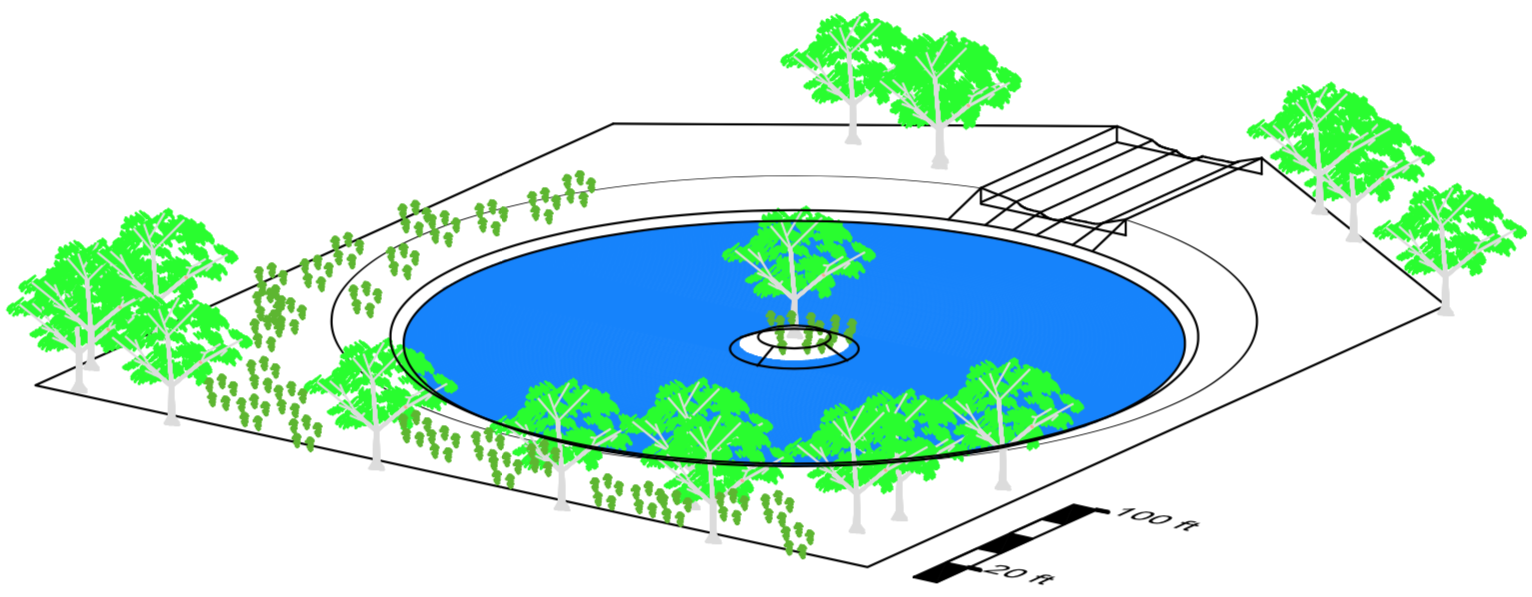
\includegraphics[height=.2\textheight]{F3P.png}
%     \caption{Impression of what the pond may look like after landscaping. }
% \end{figure}

%%%%%%%%%%%%%%%%%%%%%%%%%%%%%%%%%%%%%%%%%%%%%%%%%%%%%%%%%%%%%%%%%%
%%%%%%%%%%%%%%%%%%%%% 8.0 Required Resources %%%%%%%%%%%%%%%%%%%%%
%%%%%%%%%%%%%%%%%%%%%%%%%%%%%%%%%%%%%%%%%%%%%%%%%%%%%%%%%%%%%%%%%%

\setcounter{figure}{0}
\setcounter{section}{0}
\setcounter{table}{0}
\chapter{Required Resources}


For this project, an estimated 15 hours per week is expected from each engineer, totalling 675 person-hours over the course of 15 weeks. This includes approximately 9 individual hours per week spent in lectures, labs, and meetings. The remaining 6 hours per person per week will be spent on the tasks detailed in the project timeline in Appendix C, with some of the major tasks overlapping. A breakdown of these person hours are shown below in Table 8.1. These estimates will likely fluctuate over the course of the project. The number of hours spent each week will be adjusted as needed to meet deadlines. 

pHlux Engineering will request access from the client to conduct site visits to the UC Davis WWTP to better understand the project site and to document the current system’s features. The drafting of the technical memorandum and the design of a new disinfection system will require the use of various resources. For the technical memorandum, data from a bioassay test conducted by Carollo Engineers and historical rainfall data, provided by Carollo Engineers and the client, will be used. To design a new UV disinfection system, the historical rainfall data, most probable number data, and existing system as-builts will be requested from the client to create a new system. Various software programs will be used to analyze the data and model the final design. For example, MATLAB will be used to model and evaluate the performance of alternative disinfection designs. FlowMaster and CFD Ultimate will be used to evaluate and optimize the hydraulics of the final design. Lastly, AutoCAD will be used to draft construction drawings of the proposed disinfection system.

\begin{table}[H]
    \centering
    \caption{Breakdown of required person-hours.}

    \def\arraystretch{1}
    \begin{tabular}{c|ccc|ccc}
    
    & \multicolumn{3}{c|}{\textbf{Meetings}} & \multicolumn{3}{c}{\textbf{Major Tasks}} \\
        \textit{}&\textit{Lecture}&\textit{Lab}&\textit{Meetings}&\textit{UVT Memo}&\textit{UV Sys. Design}&\textit{Final Deliverables} \\ \hline
    hrs/person/week& 2& 3 & 2-3 & 6 (10 wks) & 6 (15 wks) & 6 (6 wks)\\ \hline
        
 

    \end{tabular} 
\end{table}


\begin{flushleft}
\newpage
\bibliography{bib} 
\addcontentsline{toc}{chapter}{References}

\bibliographystyle{ieeetr} 
\end{flushleft}


%%%%%%%%%%%%%%%%%%%%%%%%%%%%%%%%%%%%%%%%%%%%%%%%%%%%%%%%%%%
%%%%%%%%%%%%%%%%%%%%% 10.0 Appendix A %%%%%%%%%%%%%%%%%%%%%
%%%%%%%%%%%%%%%%%%%%%%%%%%%%%%%%%%%%%%%%%%%%%%%%%%%%%%%%%%%
\newpage
\setcounter{figure}{0}
\setcounter{section}{0}
\setcounter{table}{0}


\hspace{0pt}
\vfill
\begin{center}
\chapter*{Appendix A - Resumes}
\addcontentsline{toc}{chapter}{Appendix A - Resumes}
\vfill
\hspace{0pt}
\end{center}




\renewcommand{\thefigure}{A.\arabic{figure}}
\setcounter{figure}{0}

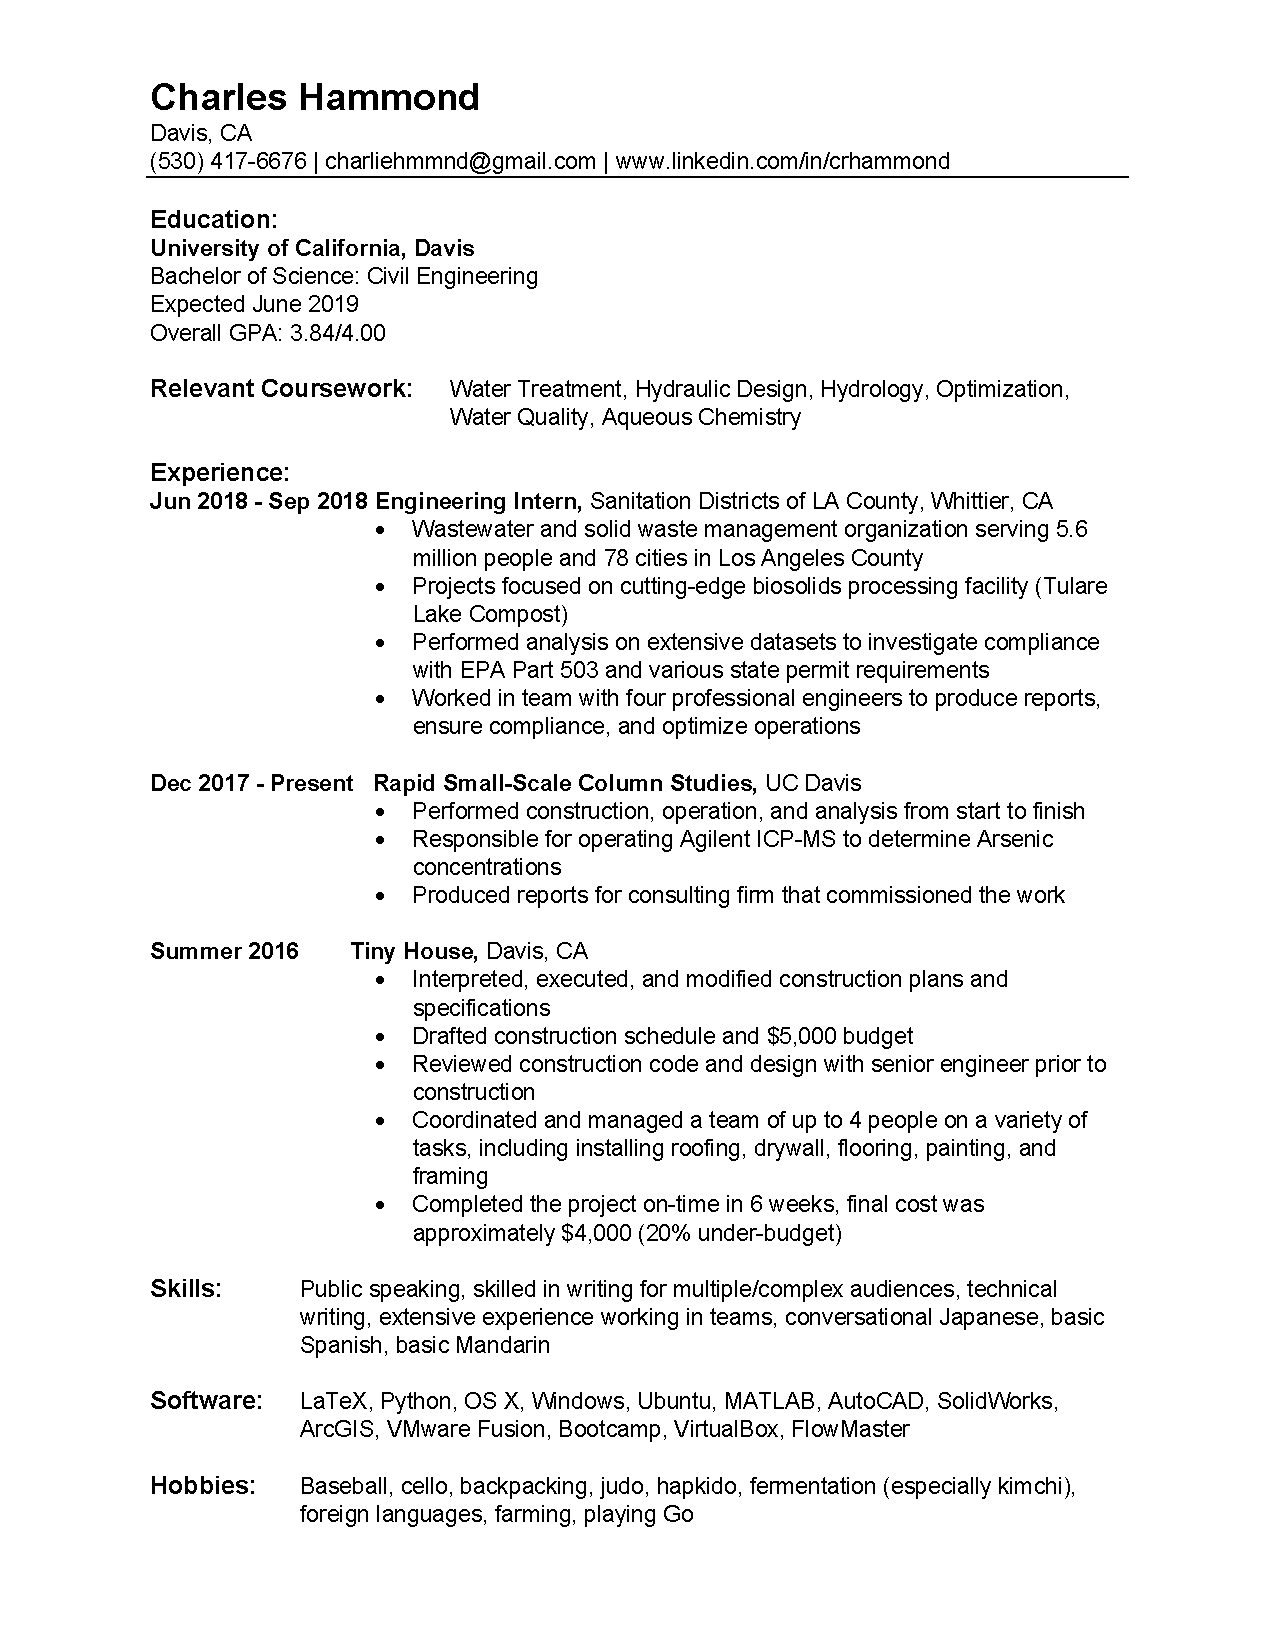
\includepdf{RCH.pdf}

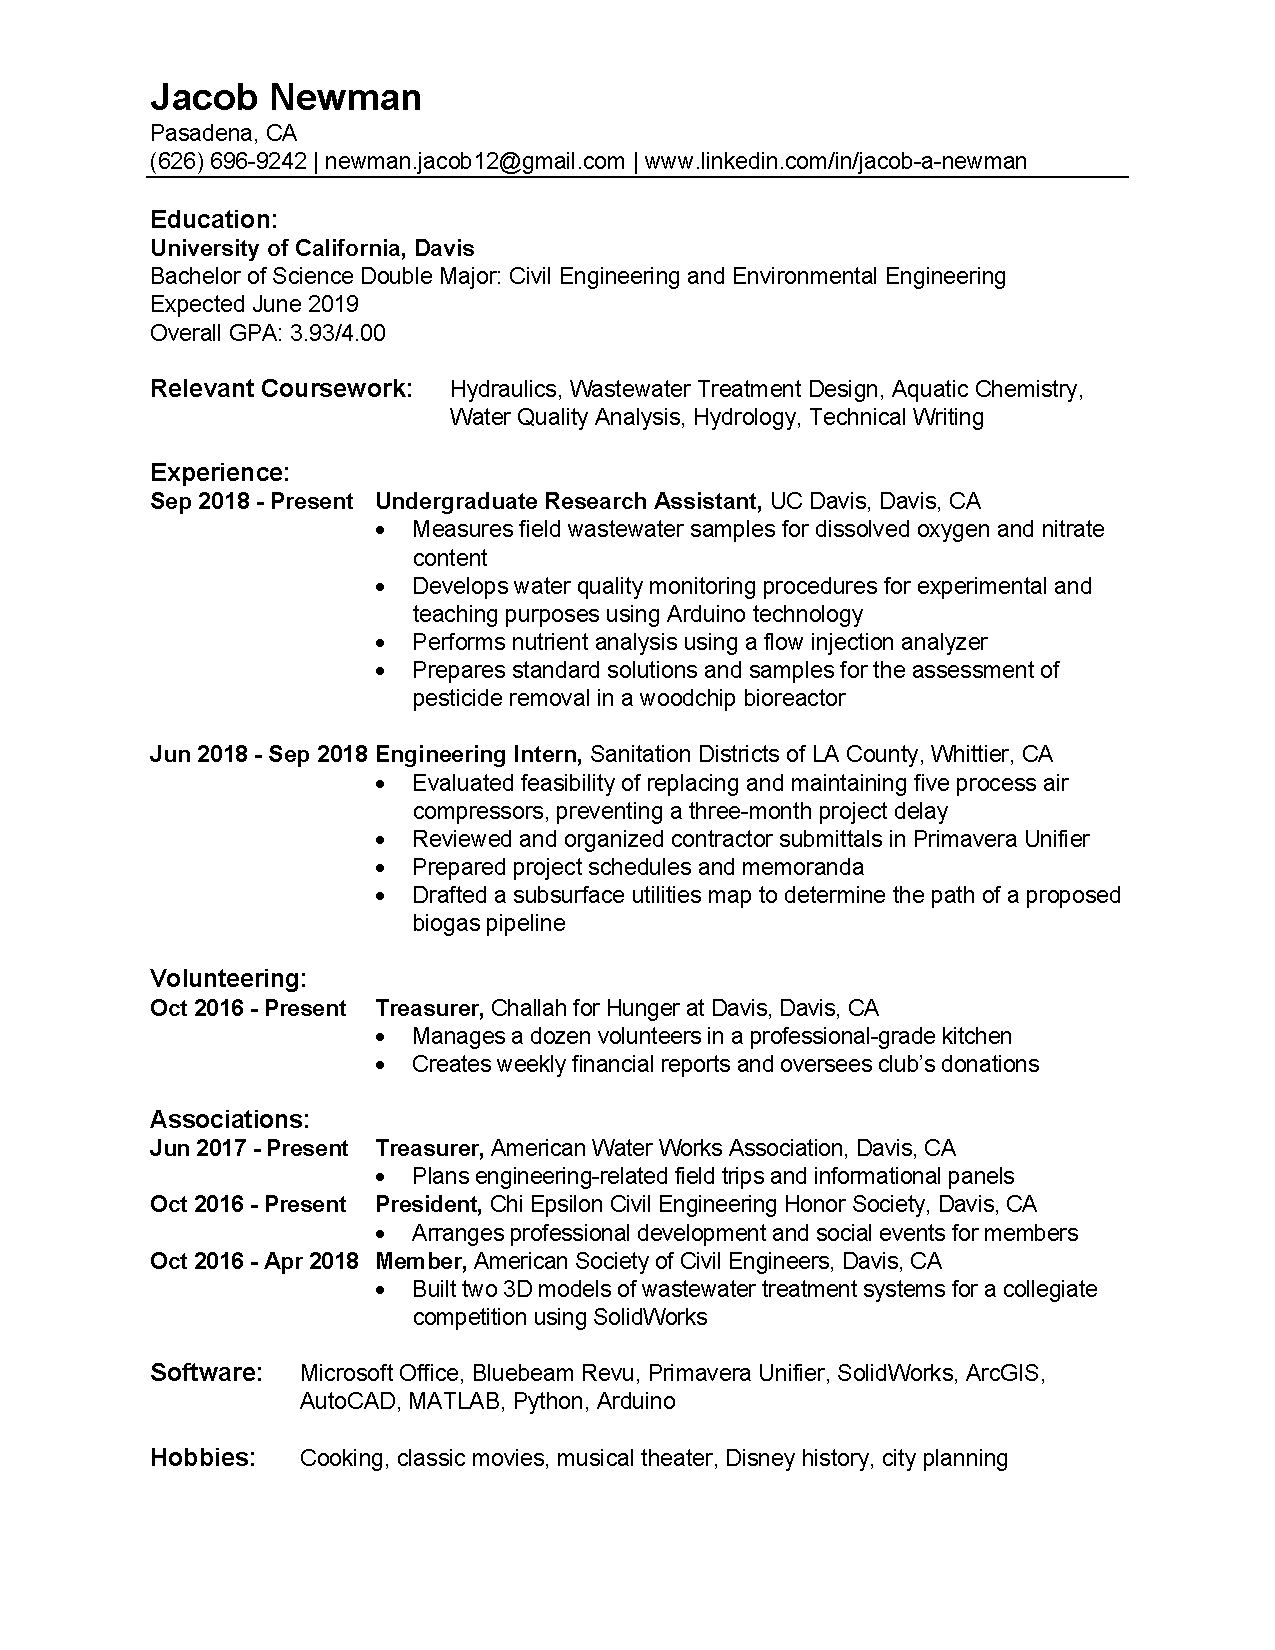
\includepdf{RJN.pdf}

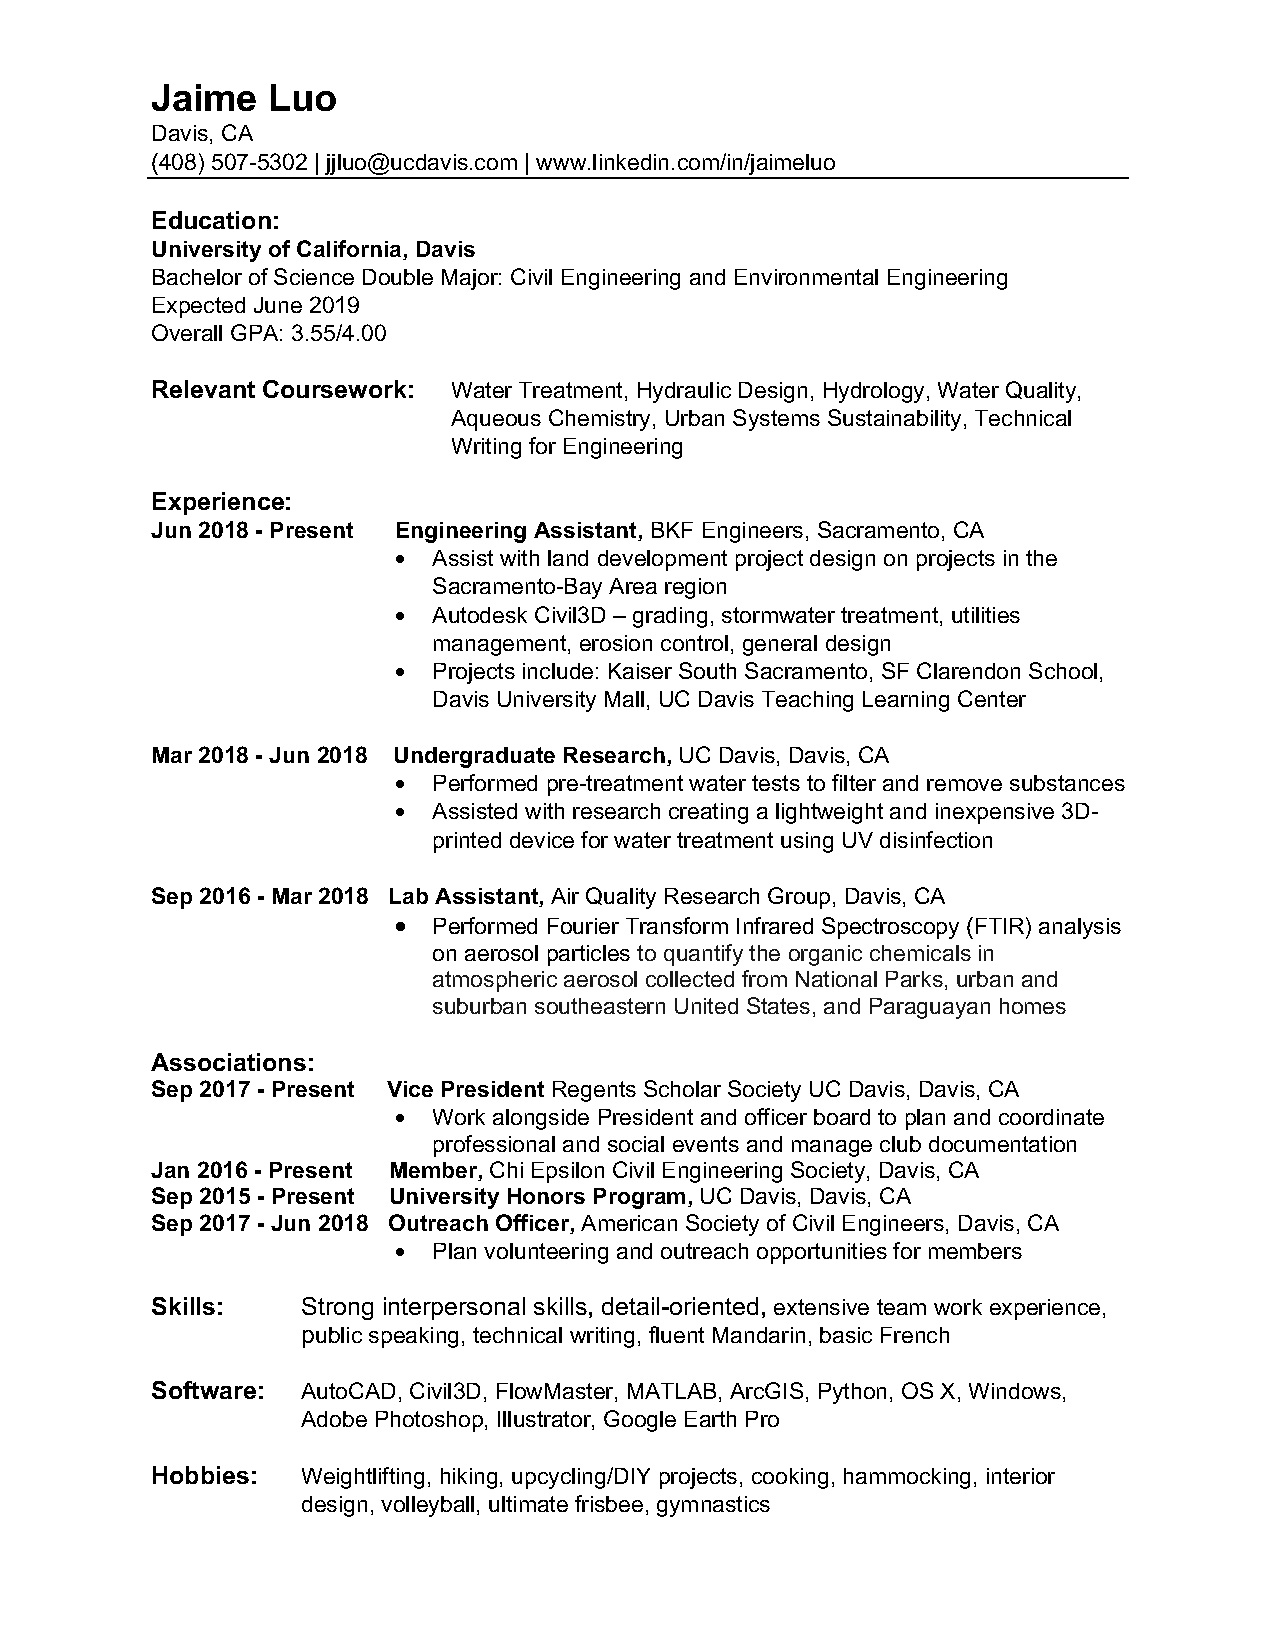
\includepdf{RJL.pdf}

\begin{landscape}
\newpage
\setcounter{figure}{0}
\setcounter{section}{0}
\setcounter{table}{0}

\chapter*{Appendix B - Assessment Criteria}

\addcontentsline{toc}{chapter}{Appendix B - Assessment Criteria}

\renewcommand{\thetable}{B.\arabic{table}}

\begin{table}[H]

    \centering
    
    \caption{Assessment criteria for alternatives.}

    \def\arraystretch{2}
    
    \begin{tabular}{lccc}

\textbf{Criteria}&\textbf{Assessment Tool}&\textbf{Performance Metric}&\textbf{Threshold for Success} \\ \hline

Capital Cost & Literature/manufacturer Estimates & Dollars to Construct & Lowest \\
O\&M Cost & Literature/manufacturer Estimates & Annual Cost of O\&M & Lowest \\
Maintenance Requirements & Literature/manufacturer Estimates & Weekly person-hours & Lowest \\
Operational Hazards & Literature/manufacturer Information & Number of safety concerns & Fewest \\
Meets Title 22 Standards & Title 22 & $\frac{\text{Standards met}}{\text{\# of standards}}$& 100\% \\
Utilizes Existing Infrastructure & Inventory of existing onsite infrastructure & Dollars saved by using existing equipment & Greatest savings \\
Energy Efficiency & Literature and manufacturer’s specifications & $\frac{\text{kWh input}}{\text{kWh output}}$ & Closest to 1 \\
Life Cycle Assessment & Literature/manufacturer Estimates & Annual Cost of O\&M & Lowest \\
Permissible UVT & Literature/manufacturer Estimates & UVT (\%) & Less than 55\% \\
System Lifetime & Literature/manufacturer Estimates & Years & $\geq 20$ \\ \hline


\end{tabular} 
\end{table}



\newpage
\setcounter{figure}{0}
\setcounter{section}{0}
\setcounter{table}{0}
\chapter*{Appendix C - Project Timeline}
\addcontentsline{toc}{chapter}{Appendix C - Project Timeline}
\renewcommand{\thefigure}{C.\arabic{figure}}


\begin{figure}[H]
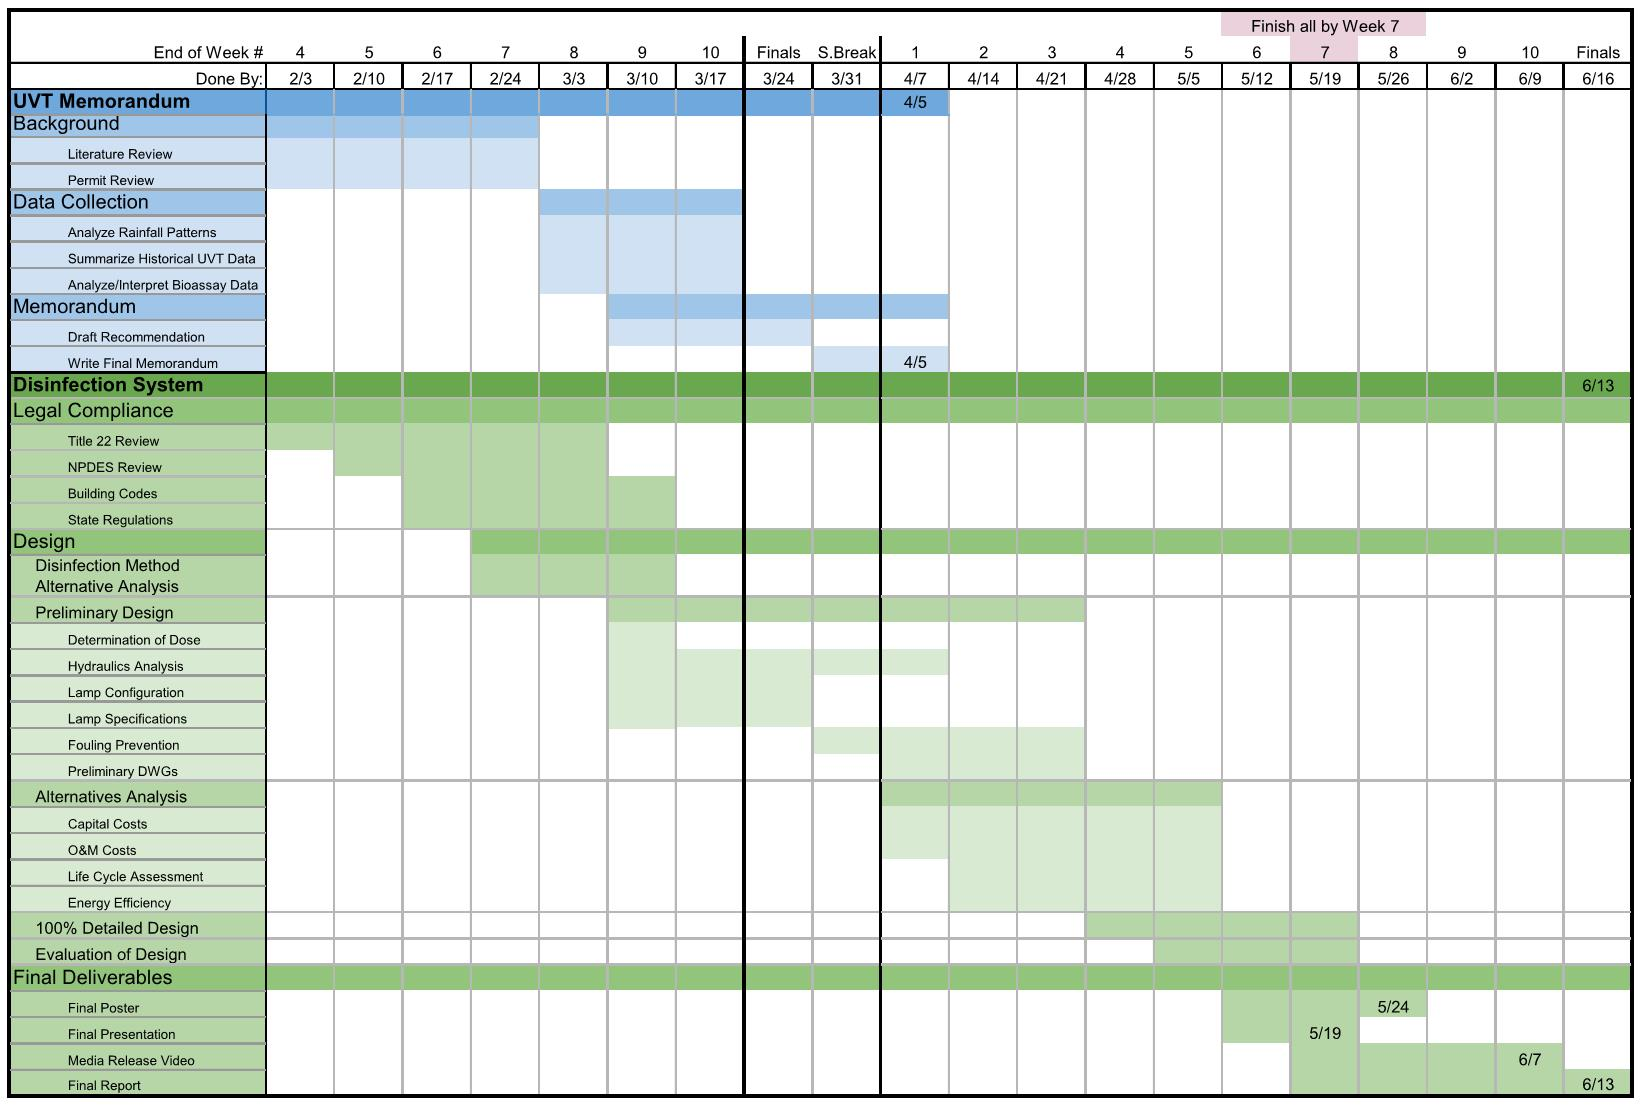
\includegraphics[height=0.95\textheight]{UV_Project_Gantt_Chart.jpg}
\centering
\caption{Gantt chart showing the project timeline.}
\setcounter{figure}{0}
\end{figure}


\newpage
\setcounter{figure}{0}
\setcounter{section}{0}
\setcounter{table}{0}
\chapter*{Appendix D - Work Breakdown Structure}
\addcontentsline{toc}{chapter}{Appendix D - Work Breakdown Structure}
\renewcommand{\thefigure}{D.\arabic{figure}}


\begin{figure}[H]
\includegraphics[height=0.85\textheight]{"UV Disinfect Work Breakdown Structure".jpg}
\centering
\caption{Work breakdown structure for UVT memorandum and disinfection system design.}
\setcounter{figure}{0}
\end{figure}
\end{landscape}





\end{document}
